%%%%%%%% DATA LITERACY 2025 LATEX PROJECT TEMPLATE FILE %%%%%%%%%%%%%%%%%
%%% Based on the 2025 ICML template, available at https://icml.cc/Conferences/2025/AuthorInstructions %%%

\documentclass{article}

% Recommended, but optional, packages for figures and better typesetting:
\usepackage{microtype}
\usepackage{graphicx}
\usepackage{subfigure}
\usepackage{booktabs} % for professional tables

\usepackage{tikz}
% Corporate Design of the University of Tübingen
% Primary Colors
\definecolor{TUred}{RGB}{165,30,55}
\definecolor{TUgold}{RGB}{180,160,105}
\definecolor{TUdark}{RGB}{50,65,75}
\definecolor{TUgray}{RGB}{175,179,183}

% Secondary Colors
\definecolor{TUdarkblue}{RGB}{65,90,140}
\definecolor{TUblue}{RGB}{0,105,170}
\definecolor{TUlightblue}{RGB}{80,170,200}
\definecolor{TUlightgreen}{RGB}{130,185,160}
\definecolor{TUgreen}{RGB}{125,165,75}
\definecolor{TUdarkgreen}{RGB}{50,110,30}
\definecolor{TUocre}{RGB}{200,80,60}
\definecolor{TUviolet}{RGB}{175,110,150}
\definecolor{TUmauve}{RGB}{180,160,150}
\definecolor{TUbeige}{RGB}{215,180,105}
\definecolor{TUorange}{RGB}{210,150,0}
\definecolor{TUbrown}{RGB}{145,105,70}

% hyperref makes hyperlinks in the resulting PDF.
% If your build breaks (sometimes temporarily if a hyperlink spans a page)
% please comment out the following usepackage line and replace
% \usepackage{icml2023} with \usepackage[nohyperref]{icml2023} above.
\usepackage{hyperref}


% Attempt to make hyperref and algorithmic work together better:
\newcommand{\theHalgorithm}{\arabic{algorithm}}

\usepackage[accepted]{icml2025}

% For theorems and such
\usepackage{amsmath}
\usepackage{amssymb}
\usepackage{mathtools}
\usepackage{amsthm}
\usetikzlibrary{arrows.meta, positioning, calc}

% if you use cleveref..
\usepackage[capitalize,noabbrev]{cleveref}

% Todonotes is useful during development; simply uncomment the next line
%    and comment out the line below the next line to turn off comments
%\usepackage[disable,textsize=tiny]{todonotes}
\usepackage[textsize=tiny]{todonotes}


% The \icmltitle you define below is probably too long as a header.
% Therefore, a short form for the running title is supplied here:
\icmltitlerunning{Exposure-Adjusted Bicycle Crash Risk Estimation and Safer Routing in Berlin} % I think our title is not too long, hence we can use the same as for \icmltitle

\begin{document}

\twocolumn[
\icmltitle{Exposure-Adjusted Bicycle Crash Risk Estimation and Safer Routing in Berlin}

% It is OKAY to include author information, even for blind
% submissions: the style file will automatically remove it for you
% unless you've provided the [accepted] option to the icml2023
% package.

% List of affiliations: The first argument should be a (short)
% identifier you will use later to specify author affiliations
% Academic affiliations should list Department, University, City, Region, Country
% Industry affiliations should list Company, City, Region, Country

% You can specify symbols, otherwise they are numbered in order.
% Ideally, you should not use this facility. Affiliations will be numbered
% in order of appearance and this is the preferred way.
\icmlsetsymbol{equal}{*}

\begin{icmlauthorlist}
\icmlauthor{Eric Berger}{equal}
\icmlauthor{Edward Eichhorn}{equal}
\icmlauthor{Liaisan Faidrakhmanova}{equal}
\icmlauthor{Luise Grasl}{equal}
\icmlauthor{Tobias Schnarr}{equal}
\end{icmlauthorlist}

% fill in your matrikelnummer, email address, degree, for each group member
% \icmlaffiliation{first}{Matrikelnummer 7064584, MSc Machine Learning}
% \icmlaffiliation{second}{Matrikelnummer 12345678, MSc Quantitative Data Science}
% \icmlaffiliation{third}{Matrikelnummer 7320172, MSc Quantitative Data Science}
% \icmlaffiliation{fourth}{Matrikelnummer 7329274, MSc Quantitative Data Science}
% \icmlaffiliation{fith}{Matrikelnummer 7304640, MSc Quantitative Data Science}

% put your email addresses here. You can use initials to save space, 
% e.g. if you are called Max Mustermann, you can use \icmlcorrespondingauthor{MM}{max.mustermann@uni-tuebingen.de}
% DO USE YOUR UNIVERSITY EMAIL ADDRESS!
% \icmlcorrespondingauthor{EB}{eric.berger@student.uni-tuebingen.de} 
% \icmlcorrespondingauthor{EE}{first2.last2@uni-tuebingen.de}
% \icmlcorrespondingauthor{LF}{liaisan.faidrakhmanova@student.uni-tuebingen.de}
% \icmlcorrespondingauthor{LG}{luise.grasl@student.uni-tuebingen.de}
\icmlcorrespondingauthor{Tobias Schnarr}{tobias-marco.schnarr@student.uni-tuebingen.de}

% You may provide any keywords that you
% find helpful for describing your paper; these are used to populate
% the "keywords" metadata in the PDF but will not be shown in the document
\icmlkeywords{Machine Learning, ICML}

\vskip 0.3in
]

% this must go after the closing bracket ] following \twocolumn[ ...

% This command actually creates the footnote in the first column
% listing the affiliations and the copyright notice.
% The command takes one argument, which is text to display at the start of the footnote.
% The \icmlEqualContribution command is standard text for equal contribution.
% Remove it (just {}) if you do not need this facility.

%\printAffiliationsAndNotice{}  % leave blank if no need to mention equal contribution
\printAffiliationsAndNotice{\icmlEqualContribution} % otherwise use the standard text.

\begin{abstract}
We investigate bicycle crash risk on Berlin’s urban street network, addressing a key limitation of many safety analyses: raw crash counts conflate danger with demand and fail to distinguish
intrinsically risky locations from high-use roads. We combine police-reported crashes with a city-wide dataset of measured bicycle volumes to compute exposure-adjusted risk at the street-segment 
and junction levels. Aggregating risk to arbitrary routes enables comparisons that trade off safety against convenience. The result is a reproducible framework for exposure-controlled bicycle 
safety analysis and routing.\todo{rewrite/edit, when we have final results}
\end{abstract}

\section{Introduction}\label{sec:intro}
\begin{figure*}[t]
  \centering
  \includegraphics{figs/map_3_panels.pdf}
  \caption{\textbf{Safety-aware routing pipeline for the Berlin cycling network.}
  Panels (a--c) are zoomed in for readability; see \cref{sec:methods} for formal definitions and notation.
  (a): Police-recorded bicycle crashes in June 2021 ({\color{TUorange}points}) and street segments with measured cyclist exposure ({\color{TUgray}lines}, used as the base network in all panels).
  (b): Pooled segment-level relative crash risk estimated from all available data; high-risk segments in {\color{TUred}red} correspond to the top 90th percentile of relative risk. {\color{TUdark}Circles} mark junctions (degree $\ge 3$), for which we also estimate junction-level relative risk from exposure aggregated over incident segments.
  (c): Shortest path ({\color{TUblue}blue}) versus a safer alternative ({\color{TUgreen}green}) selected to reduce cumulative relative route risk under a distance-detour constraint. {\color{TUocre}Filled circle} and {\color{TUocre}cross} denote origin and destination, respectively; {\color{TUdark}circles} show junctions for reference.
  }
  \label{fig:visual_app}
\end{figure*}

% Cycling safety analyses often rely on raw crash counts, which conflate danger with demand: streets that attract many cyclists tend to accumulate more incidents even when per-rider risk is 
% low~\citep{luecken2018}. This obscures intrinsically risky locations and limits both targeted interventions and everyday route choice, especially in dense urban networks such as Berlin~\citep{Uijtdewilligen01092024}.
% We address this by estimating exposure-adjusted crash risk on the street network via a relative-risk formulation that separates cyclist demand from intrinsic danger and remains stable under sparse 
% or unevenly distributed observations (\cref{sec:methods}). The resulting estimates are transformed into expected crash costs and propagated to route-level scores suitable for navigation. Our study combines police-recorded 
% crashes from the German Unfallatlas (Berlin subset)~\citep{Unfallatlas2025} with a city-wide dataset of measured bicycle volumes at the street-segment level~\citep{kaiser_2025_15332147}. We compute 
% exposure-adjusted relative risk for individual street segments and, motivated by the concentration of crashes at intersections, derive junction-level risk by aggregating volumes from adjoining segments. 
% We then aggregate segment- and junction-level expected crash costs to evaluate arbitrary routes and compare alternatives that reduce estimated risk while maintaining comparable convenience in terms 
% of distance or travel time, see \cref{fig:visual_app}. We address the question: how can exposure-adjusted relative crash risk be estimated from measured bicycle volumes and integrated into safety-aware
% routing? Our work makes the following contributions: (i) a reproducible pipeline for estimating exposure-adjusted relative crash risk at street and junction levels from measured cyclist volumes; and 
% (ii) a route-scoring method that integrates network-level risk into safety-aware routing under convenience constraints.

Cycling safety analyses often rely on raw crash counts, which conflate danger with demand: streets that attract many cyclists tend to accumulate more incidents even when per-rider risk is 
low~\citep{luecken2018}. This obscures intrinsically risky locations and limits both targeted interventions and everyday route choice, especially in dense urban networks such as Berlin~\citep{Uijtdewilligen01092024}.
We address this by estimating exposure-adjusted crash risk on the street network via a relative-risk formulation that separates cyclist demand from intrinsic danger and remains stable under sparse
or unevenly distributed observations (\cref{sec:methods}). Using police-recorded crashes from the German Unfallatlas (Berlin subset)~\citep{Unfallatlas2025} together with a city-wide dataset of 
measured bicycle volumes at the street-segment level~\citep{kaiser_2025_15332147}, we compute exposure-adjusted relative risk for individual street segments and, motivated by the concentration of
crashes at intersections, derive junction-level risk by aggregating volumes from adjoining segments. The resulting risk estimates are transformed into expected crash costs and propagated to route-level 
scores, enabling the evaluation of arbitrary routes and comparisons between alternatives that reduce estimated risk while maintaining comparable convenience in terms of distance (\cref{sec:results}), 
see \cref{fig:visual_app}.

Taken together, this yields a reproducible pipeline for estimating exposure-adjusted crash risk at street and junction levels from measured cyclist volumes, and a route-scoring approach that 
integrates network-level risk into safety-aware routing under a bounded detour constraint.

\section{Data}\label{sec:data}
% In this section, describe \emph{what you did}. Roughly speaking, explain what data you worked with, how or from where it was collected, it's structure and size. Explain your analysis, and any specific choices you made in it. Depending on the nature of your project, you may focus more or less on certain aspects. If you collected data yourself, explain the collection process in detail. If you downloaded data from the net, show an exploratory analysis that builds intuition for the data, and shows that you know the data well. If you are doing a custom analysis, explain how it works and why it is the right choice. If you are using a standard tool, it may still help to briefly outline it. Cite relevant works. You can use the \verb|\citep| and \verb|\citet| commands for this purpose \citep{mackay2003information}.
We combine police-recorded bicycle crashes with measured cyclist exposure for the city of Berlin. Crash data are drawn from the Berlin subset of the German \emph{Unfallatlas}~\citep{Unfallatlas2025} 
and filtered for bicycle-related incidents. Exposure comes from a city-wide dataset of measured bicycle volumes aggregated at the street-segment level~\citep{kaiser2025spatiotemporalgraphneuralnetwork}.
We further evaluate how well cyclist volumes derived from Strava align with measurements from official bicycle counting stations (see \cref{fig:segment_share}).
The street network is represented as polyline segments with associated monthly cyclist counts. The resulting dataset spans 2019--2023 and covers 4{,}335 street segments and 2{,}862 junctions, 
with 15{,}396 recorded bicycle crashes. At monthly resolution the data are sparse: in a typical month fewer than 5\% of segments and about 3\% of junctions record at least one crash, and 
some periods include segments with zero measured exposure.\todo{verify the percentages}

\begin{figure}[h]
  \centering
  \includegraphics{figs/segment_share.pdf}
  \caption{Alignment between official bicycle counts and Strava-derived cyclist volumes at the street-segment level in 2023. Points show segment-wise shares of total annual counts, with the dashed line indicating perfect agreement between the two sources.}
  \label{fig:segment_share}
\end{figure}

To enable network-scale analysis, all layers are harmonized to a common street-network topology and a projected coordinate reference system. Crash locations are matched to segments using 
nearest-segment assignment. To capture the concentration of crashes at intersections, we identify junctions as nodes where at least three segments meet; crashes within a fixed radius are 
assigned to the nearest junction, and junction exposure is computed from the exposures of incident segments. Matched crashes and exposures are aggregated to monthly resolution, and segments 
and months with zero exposure are dropped. To obtain stable risk estimates under sparse observations, monthly aggregates are pooled to yearly totals and an Empirical Bayes 
approach is applied as described in \cref{sec:methods}. The resulting yearly segment- and junction-level risk estimates serve as inputs to all routing analyses.

\section{Methods}\label{sec:methods}
\paragraph{Empirical Bayes relative risk.}
For each month $t$, let $A_{s,t}$ and $E_{s,t}$ denote the number of police-recorded bicycle crashes and the measured cyclist exposure on street segment $s$. Junction crashes
$A_{v,t}$ are defined as crashes occurring within a fixed radius of the centroid of junction $v$. Because a traversal typically contributes exposure to two incident segments, 
entering and exiting, we approximate junction exposure by a half-sum of incident segment exposures,
\[
E_{v,t}=\tfrac{1}{2}\sum_{s\in\mathcal I(v)} E_{s,t},
\]
which avoids double-counting. Aggregating exposure over incident links is common when turning movements are unavailable~\citep{hakkert2002uses,WANG2020105838}.

For notational convenience, we index both street segments and junctions by a generic entity index $i$, with $A_{i,t}$ and $E_{i,t}$ denoting the corresponding crash and exposure 
quantities.

We assume that, within a given month, crash incidence is proportional to exposure under a ``no special risk'' baseline. This yields the expected number of crashes
\[
\widehat{A}_{i,t}
= A_{\cdot t}\,\frac{E_{i,t}}{E_{\cdot t}},
\qquad
A_{\cdot t}=\sum_{i} A_{i,t},\ \ E_{\cdot t}=\sum_{i} E_{i,t},
\]
where sums are taken over all segments and junctions. Segment-level and junction-level crashes are disjoint by construction, so the pooled totals $A_{\cdot t}$ and $E_{\cdot t}$ define a shared baseline.

Although crashes and exposure are aggregated at monthly resolution in preprocessing, routing requires a stable long-run risk surface. We therefore pool monthly quantities across the full study period to obtain
\[
A_i=\sum_t A_{i,t},
\qquad
E_i=\sum_t E_{i,t},
\]
and define the corresponding baseline expectation
\[
\widehat{A}_i
= A_\cdot\,\frac{E_i}{E_\cdot},
\qquad
A_\cdot=\sum_i A_i,\ \ E_\cdot=\sum_i E_i.
\]

To stabilize estimation under sparse observations, we introduce a latent relative-risk multiplier $\theta_i$ and model
\[
A_i \mid \theta_i \sim \text{Poisson}(\widehat{A}_i\,\theta_i),
\qquad
\theta_i \sim \text{Gamma}(\alpha,\alpha),
\]
where the Gamma distribution is parameterized in shape--rate form, enforcing a unit prior mean $\mathbb{E}[\theta_i]=1$. The hyperparameter $\alpha$ is estimated from the pooled data using a method-of-moments estimator. By conjugacy, the posterior mean
\[
r_i
= \mathbb{E}[\theta_i \mid A_i,\widehat{A}_i]
= \frac{A_i+\alpha}{\widehat{A}_i+\alpha}
\]
serves as our Empirical Bayes smoothed relative risk. This estimator shrinks extreme values toward $1$, with stronger shrinkage for entities with low expected crash counts.

\paragraph{Risk rescaling for routing.}
Relative risk estimates are dimensionless and reflect risk conditional on exposure. To obtain additive weights suitable for routing, we rescale relative risk by the pooled baseline crash rate
\[
\bar{\lambda}=\frac{A_\cdot}{E_\cdot}.
\]
The resulting entity-level routing weight is
\[
w_i=\bar{\lambda}\,r_i,
\]
which can be interpreted as an exposure-adjusted crash rate up to a global constant. This rescaling preserves relative differences in risk while yielding quantities that aggregate naturally along routes.

\paragraph{Routing graph.}
We build an undirected graph $G=(V,E)$ from the street network. Nodes represent segment endpoints and edges represent street segments with length $\ell_e$. Each graph edge $e$ corresponds to a street segment $s$ and inherits its routing weight, denoted $w_e=w_s$. Junction identifiers and weights are mapped to nodes via spatial snapping in a projected coordinate system, yielding a single risk-annotated network.

\paragraph{Safety-aware routing.}
We compare shortest-distance routes with alternatives that reduce estimated crash risk under a bounded detour. The length of a route $P$ is
\[
L(P)=\sum_{e\in P}\ell_e.
\]
To account for both segment-level and junction-level risk, the risk contribution of edge $e=(u,v)$ is defined as
\[
\rho_e = w_e + \eta\,\frac{w_u+w_v}{2},
\]
where $w_u$ and $w_v$ are junction routing weights, set to zero for non-junction nodes, and $\eta\ge 0$ controls the contribution of junction risk. We interpret these quantities as an additive surrogate for cumulative route risk, not as probabilities.

Given an origin--destination pair, the baseline route $P_{\text{dist}}$ minimizes $L(P)$. The safety-aware route solves
\begin{equation}
\label{eq:safe-routing}
\begin{aligned}
P_{\text{safe}}=\arg\min_{P}\ & R(P)=\sum_{e\in P}\rho_e \\
\text{s.t.}\ & L(P)\le (1+\varepsilon)\,L(P_{\text{dist}}),
\end{aligned}
\end{equation}
where $\varepsilon$ is the allowable relative detour~\citep{ehrgott2005multicriteria}. We approximate this constrained problem using a weighted-sum sweep. For $\lambda\in\Lambda$,
\[
P(\lambda)=\arg\min_{P}\sum_{e\in P}\bigl(\rho_e+\lambda\,\ell_e\bigr),
\]
then select among feasible candidates the route with minimal $R(P)$, breaking ties by shorter $L(P)$. Shortest paths are computed using Dijkstra’s algorithm.

\paragraph{Evaluation metrics.}
For each origin--destination pair, we report the relative length increase
\[
\Delta_L=\frac{L(P_{\text{safe}})-L(P_{\text{dist}})}{L(P_{\text{dist}})}
\]
and the relative risk reduction
\[
\Delta_R=\frac{R(P_{\text{dist}})-R(P_{\text{safe}})}{R(P_{\text{dist}})}.
\]
Pairs with $R(P_{\text{dist}})=0$ are excluded from $\Delta_R$ due to an undefined denominator. These metrics quantify how bounded detours trade distance for reductions in exposure-adjusted crash risk.

\section{Related work.}\label{sec:relatedw}
Prior work has aimed to avoid conflating danger with demand by normalizing bicycle crashes by cyclist exposure~\citep{luecken2018}. City-scale studies demonstrate that exposure-normalized risk 
yields more informative spatial patterns than raw crash counts, and that finer temporal resolution improves inference, though persistent under-reporting in police records remains a challenge~\citep{Uijtdewilligen01092024}. 
A central obstacle in this line of research is obtaining reliable exposure: earlier methods extrapolate city-wide volumes from sparse counters using learning-based models and multi-source features, 
while short-term measurement campaigns improve predictions at unseen locations~\citep{Kaiser_Klein_Kaack_2025}. More recent efforts leverage street-segment datasets of measured bicycle volumes, 
enabling downstream safety analyses without the need to model exposure~\citep{kaiser2025spatiotemporalgraphneuralnetwork}. At the network level, studies define risk as crashes per unit exposure 
on links and address practical challenges such as spatial snapping of crash events, assigning incidents to intersections, and integrating safety metrics into routing under convenience 
constraints~\citep{isprs-archives-XLIII-B4-2022-427-2022}. The role of intersection safety is emphasized across multiple studies, which document strong crash concentrations at junctions and 
highlight the importance of controlling for exposure when comparing infrastructure types or locations~\citep{futuretransp1030037}.

% How to make a figure
% \begin{figure}[ht]
% \vskip 0.2in
% \begin{center}
% \centerline{\includegraphics[width=\columnwidth]{figures/teacher-student.pdf}}
% \caption{Historical locations and number of accepted papers for International
% Machine Learning Conferences (ICML 1993 -- ICML 2008) and International
% Workshops on Machine Learning (ML 1988 -- ML 1992). At the time this figure was
% produced, the number of accepted papers for ICML 2008 was unknown and instead
% estimated.}
% \label{icml-historical}
% \end{center}
% \vskip -0.2in
% \end{figure}

\section{Results}\label{sec:results}

One of the major outcomes of this work ist the estimation of the risk to have get injured in a bike accidents while driving on a streetsegment.
This distribution of those calculated risks is displayed in Figure~\ref{fig:risk_segments}.


\begin{figure}[h]
  \centering
  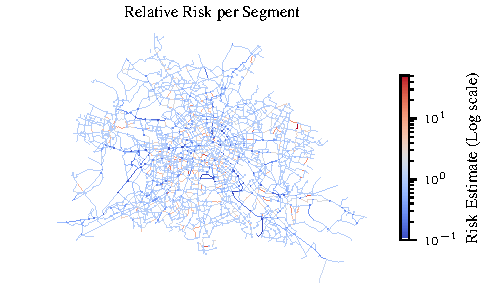
\includegraphics{figs/risk_segments.pdf}
  \caption{Risk per segment for the area of Berlin. The colors indicate the log-scaled risk for each plotted segment and junction.}
  \label{fig:risk_segments}
\end{figure}




% In this section outline your results. At this point, you are just stating the outcome of your analysis. You can highlight important aspects (``we observe a significantly higher value of $x$ over $y$''), but leave interpretation and opinion to the next section. This section absoultely \emph{must} include at least two figures.
To evaluate the routing algorithm, we sample $n=1000$ origin--destination pairs uniformly at random and compare shortest-distance routes with safety-aware alternatives \citep{NateraOrozco2020}.


\begin{table}[t]
\centering
\caption{Distance--risk trade-off under bounded detours for different junction-risk weights $\eta$.
Values are aggregated over all origin--destination pairs. Medians are reported with interquartile
ranges in parentheses.}
\label{tab:routing_tradeoff}
\begin{tabular}{@{}c c c c c@{}}
\toprule
$\eta$ & $\varepsilon$ & Med.\ $\Delta_L$ & Med.\ $\Delta_R$ & $P(\Delta_R>0)$ \\
\midrule
0.0 & 0.05 & 0.009 (0.026) & 0.246 (0.451) & 76.1 \\
    & 0.10 & 0.025 (0.042) & 0.377 (0.388) & 86.0 \\
    & 0.20 & 0.038 (0.072) & 0.425 (0.353) & 90.6 \\
\addlinespace
0.5 & 0.05 & 0.008 (0.026) & 0.208 (0.401) & 75.3 \\
    & 0.10 & 0.026 (0.046) & 0.331 (0.370) & 86.4 \\
    & 0.20 & 0.047 (0.089) & 0.404 (0.323) & 92.0 \\
\addlinespace
1.0 & 0.05 & 0.008 (0.026) & 0.185 (0.363) & 75.9 \\
    & 0.10 & 0.028 (0.047) & 0.305 (0.345) & 86.3 \\
    & 0.20 & 0.050 (0.086) & 0.378 (0.318) & 91.8 \\
\bottomrule
\end{tabular}
\end{table}

\cref{tab:routing_tradeoff} summarizes the trade-off between route length and exposure-adjusted crash risk under bounded detours. Safety-aware routing identifies feasible alternatives for all 
origin--destination pairs across detour budgets and junction-risk weights.

Allowing a 10\% detour reduces exposure-adjusted crash risk by 31--38\% in median, with over 86\% of routes achieving a risk reduction for all values of the junction-risk weight. Larger detours 
further increase these gains, reaching median reductions of 38--43\% at $\varepsilon=0.20$, while even small detours ($\varepsilon=0.05$) yield measurable reductions of 18--25\%. Across all detour
budgets, increasing $\eta$ is associated with lower median risk reductions.


\section{Discussion and Conclusion}\label{sec:conclusion}
% Use this section to briefly summarize the entire text. Highlight limitations and problems, but also make clear statements where they are possible and supported by the analysis. 
Our results indicate that substantial reductions in exposure-adjusted crash risk can be achieved with relatively small increases in route length. While higher junction-risk weights reduce the magnitude
 of the estimated risk reduction, the distance--risk trade-off persists across all configurations, with absolute gains depending on the chosen weighting.

Overall, allowing a 10\% increase in route length yields median exposure-adjusted risk reductions of 31--38\% for the majority of routes, demonstrating that safety-aware routing can effectively trade 
modest detours for meaningful safety improvements.


We provide implementation details, hyperparameters, and supplementary material, available at \url{https://github.com/ytobiaz/data_literacy}.

\clearpage

\section*{Contribution Statement}
Explain here, in one sentence per person, what each group member contributed. For example, you could write: Max Mustermann collected and prepared data. Gabi Musterfrau and John Doe performed the data analysis. Jane Doe produced visualizations. All authors will jointly wrote the text of the report. Note that you, as a group, a collectively responsible for the report. Your contributions should be roughly equal in amount and difficulty.

% \section*{Notes} 
% Your entire report has a \textbf{hard page limit of 4 pages} excluding references and the contribution statement. (I.e. any pages beyond page 4 must only contain the contribution statement and references). Appendices are \emph{not} possible. But you can put additional material, like interactive visualizations or videos, on a githunb repo (use \href{https://github.com/pnkraemer/tueplots}{links} in your pdf to refer to them). Each report has to contain \textbf{at least three plots or visualizations}, and \textbf{cite at least two references}. More details about how to prepare the report, inclucing how to produce plots, cite correctly, and how to ideally structure your github repo, will be discussed in the lecture, where a rubric for the evaluation will also be provided.


\bibliography{bibliography}
\bibliographystyle{icml2025}

\end{document}

% This document was modified from the files available at https://icml.cc/Conferences/2025/AuthorInstructions
% the full copyright notice is available within the file icml2025.sty